\paragraph{curve-scalar}

\subparagraph{Target}
Implement the multiplication between scalar and point.

\subparagraph{Constraints logic}
See \figref{fig:curve-scalar}.
\begin{figure}[!ht]
    \centering
    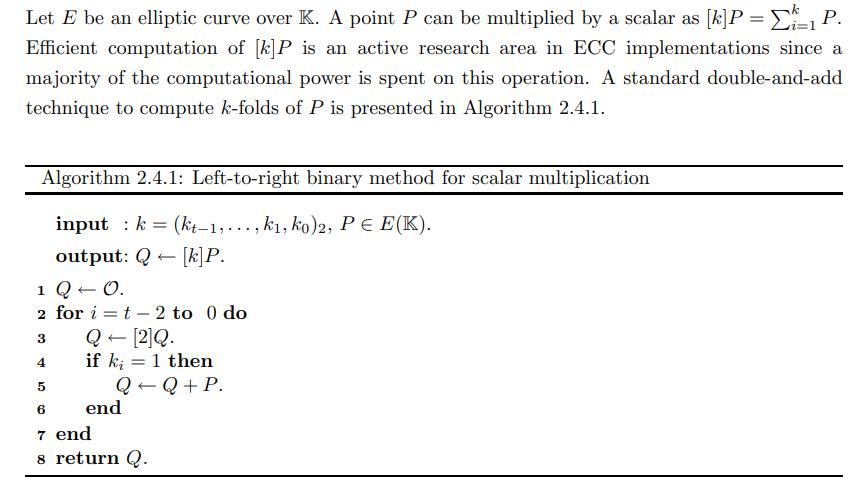
\includegraphics[width=0.5\textwidth]{curve-scalar.jpg}
    \caption{curve-scalar}
    \label{fig:curve-scalar}
\end{figure}

\subparagraph{Constraints info and costs}
\begin{itemize}
    \item gate type num: 13 
    \item gate instance num: 180364          
\end{itemize}
